\begin{description}
    \item[Umkehrbarkeit] (im engeren sinne) $f : A \longrightarrow B$
    \begin{gather*}
        \leftrightarrow (\exists g : B \longrightarrow A) g \circ f = id_A \wedge f \cdot g = id_B\\
        (\forall a \in A)\ g(f(a)) = a\\
        (\forall b \in B)\ f(g(b)) = b\\
    \end{gather*}
    Die Funktion $g : B \longrightarrow A$ heißt dann Umkehrfunktion von f, geschrieben $g = f^{-1}$.
    \[f^{-1} \not = (f)^{-1}\]
    Satz: Eine Funktion $f : A \longrightarrow B$ ist genau dann umkehrbar (i.e.s), wenn sie bijektiv ist.
    \item[Umkehrbarkeit in der Analysis] Eine Funktion $f : A \longrightarrow B$ heißt Umkehrbar, wenn die zugehörige Funktion $f : A \longrightarrow \textrm{Bild}(f)$ umkehrbar ist.
    Satz: Eine Funktion $f : A \longrightarrow B$ ist genau dann umkehrbar (i.w.s), wenn sie injektiv ist.
\end{description}

\subsubsection{Potenzfunktion}
\[f : \mathbb{R} \longrightarrow \mathbb{R},\ x \longmapsto x^n\]
\begin{description}
    \item[quadratisch] \
    \begin{tabular}[t]{cc}
        $f : \mathbb{R} \longrightarrow \mathbb{R},\ x \longmapsto x^2$ & $f^{*-1} : \mathbb{R}_0^+ \longrightarrow \mathbb{R},\ x \longmapsto \sqrt{x}$ \\
        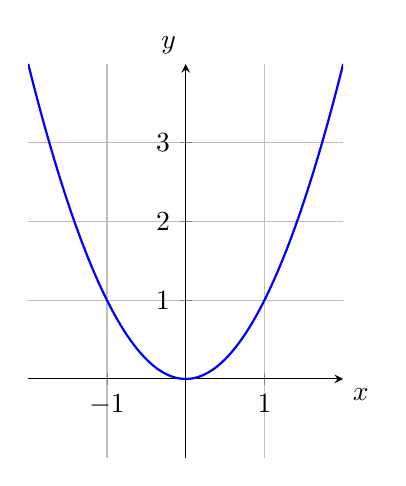
\begin{tikzpicture}
            %! suppress = Ellipsis
            \begin{axis}
                [
                x = 1cm, y = 1cm,
                xmin = -2, xmax = 2,
                ymin = -1, ymax = 4,
                axis lines = center,
                xtick={-1,0,...,1},
                ytick={0,1,...,3},
                xlabel={$x$},
                ylabel={$y$},
                xlabel style={below right},
                ylabel style={above left},
                grid=both]
                \addplot[
                    domain = -2:2,
                    samples = 200,
                    smooth,
                    thick,
                    blue,
                ] {x^2};
            \end{axis}
        \end{tikzpicture}                                               &
        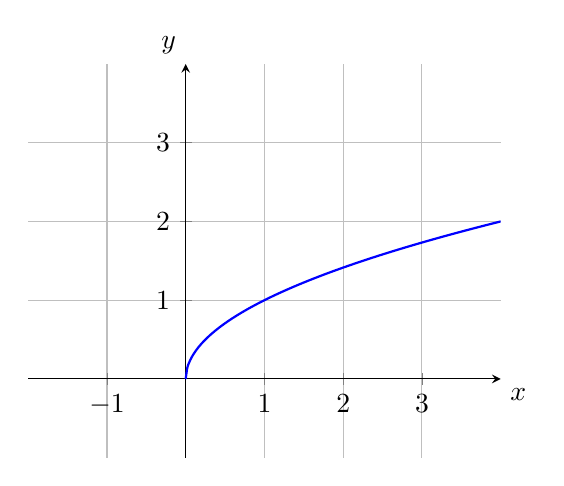
\begin{tikzpicture}
            %! suppress = Ellipsis
            \begin{axis}
                [
                x = 1cm, y = 1cm,
                xmin = -2, xmax = 4,
                ymin = -1, ymax = 4,
                axis lines = center,
                xtick={-1,0,...,3},
                ytick={0,1,...,3},
                xlabel={$x$},
                ylabel={$y$},
                xlabel style={below right},
                ylabel style={above left},
                grid=both]
                \addplot[
                    domain = 0:4,
                    samples = 200,
                    smooth,
                    thick,
                    blue,
                ] {sqrt(x)};
            \end{axis}
        \end{tikzpicture}
    \end{tabular}
    \item[kubisch] \
    \begin{tabular}[t]{cc}
        $f : \mathbb{R} \longrightarrow \mathbb{R},\ x \longmapsto x^3$ & $f^{-1} : \mathbb{R} \longrightarrow \mathbb{R},\ x \longmapsto \sqrt[3]{x}$ \\
        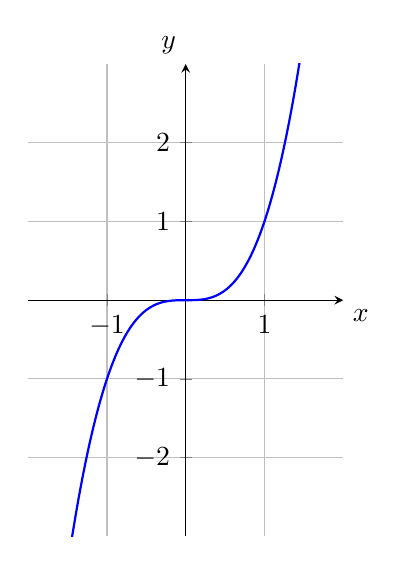
\begin{tikzpicture}
            %! suppress = Ellipsis
            \begin{axis}
                [
                x = 1cm, y = 1cm,
                xmin = -2, xmax = 2,
                ymin = -3, ymax = 3,
                axis lines = center,
                xtick={-1,0,...,1},
                ytick={-2,-1,...,2},
                xlabel={$x$},
                ylabel={$y$},
                xlabel style={below right},
                ylabel style={above left},
                grid=both]
                \addplot[
                    domain = -2:2,
                    samples = 200,
                    smooth,
                    thick,
                    blue,
                ] {x^3};
            \end{axis}
        \end{tikzpicture}                                               &
        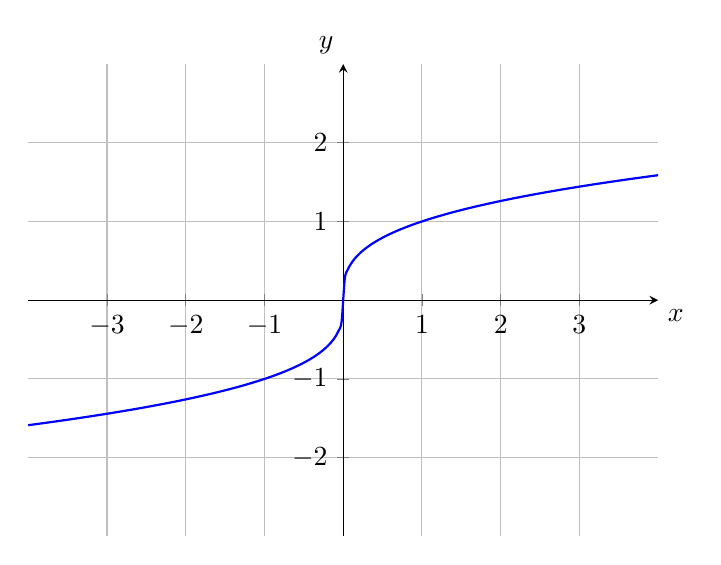
\begin{tikzpicture}
            %! suppress = Ellipsis
            \begin{axis}
                [
                x = 1cm, y = 1cm,
                xmin = -4, xmax = 4,
                ymin = -3, ymax = 3,
                axis lines = center,
                xtick={-3,-2,...,3},
                ytick={-2,-1,...,2},
                xlabel={$x$},
                ylabel={$y$},
                xlabel style={below right},
                ylabel style={above left},
                grid=both]
                \addplot[
                    domain = -4:4,
                    samples = 200,
                    smooth,
                    thick,
                    blue,
                ] {sign(x) * abs(x)^(1/3)};
            \end{axis}
        \end{tikzpicture}
    \end{tabular}
\end{description}


\subsubsection{Exponentialfunktionen}
\[f : \mathbb{R} \longrightarrow \mathbb{R}^+,\ x \longmapsto b^x \ | b \in \mathbb{R}^+ \setminus \lbrace 1 \rbrace\]
\begin{tabular}[t]{cc}
    $f : \mathbb{R} \longrightarrow \mathbb{R}^+,\ x \longmapsto 2^x$ & $f*^{-1} : \mathbb{R}^+ \longrightarrow \mathbb{R},\ x \longmapsto \log_2(x)$ \\
    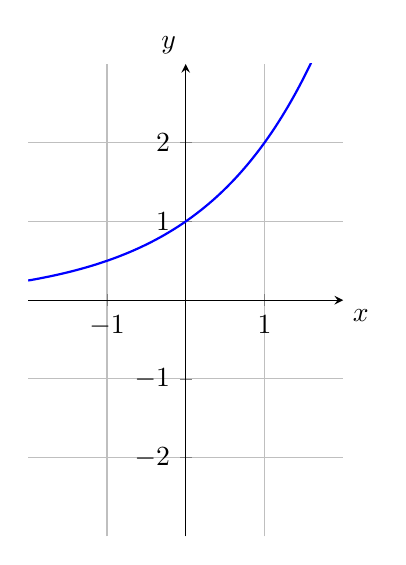
\begin{tikzpicture}
        %! suppress = Ellipsis
        \begin{axis}
            [
            x = 1cm, y = 1cm,
            xmin = -2, xmax = 2,
            ymin = -3, ymax = 3,
            axis lines = center,
            xtick={-1,0,...,1},
            ytick={-2,-1,...,2},
            xlabel={$x$},
            ylabel={$y$},
            xlabel style={below right},
            ylabel style={above left},
            grid=both]
            \addplot[
                domain = -2:2,
                samples = 200,
                smooth,
                thick,
                blue,
            ] {2^x};
        \end{axis}
    \end{tikzpicture}                                                 &
    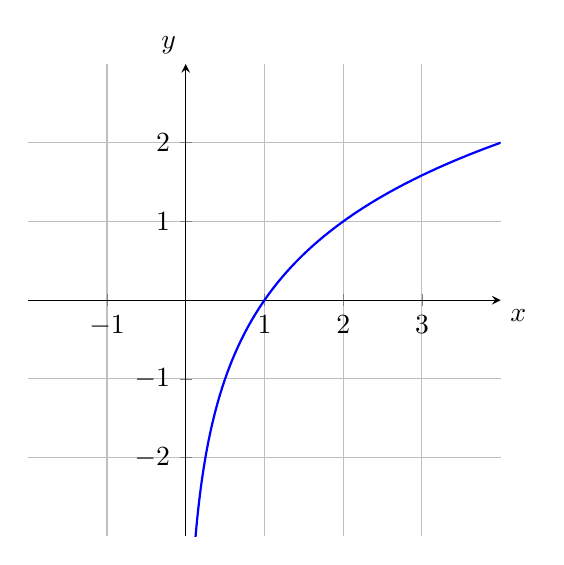
\begin{tikzpicture}
        %! suppress = Ellipsis
        \begin{axis}
            [
            x = 1cm, y = 1cm,
            xmin = -2, xmax = 4,
            ymin = -3, ymax = 3,
            axis lines = center,
            xtick={-1,0,...,3},
            ytick={-2,-1,...,2},
            xlabel={$x$},
            ylabel={$y$},
            xlabel style={below right},
            ylabel style={above left},
            grid=both]
            \addplot[
                domain = -0.01:4,
                samples = 200,
                smooth,
                thick,
                blue,
            ] {ln(x)/ln(2)};
        \end{axis}
    \end{tikzpicture}
\end{tabular}

